\documentclass[12pt,a4paper,fleqn]{article}
\usepackage[utf8]{inputenc}
\usepackage[russian]{babel}
\usepackage{amssymb, amsmath, multicol}
\usepackage{enumitem}
\usepackage{lipsum}
\usepackage{euler}
\oddsidemargin=-15.4mm
\textwidth=190mm
\headheight=-32.4mm
\textheight=277mm
\parindent=0pt
\parskip=8pt
\pagestyle{empty}
\usepackage{graphicx}
\begin{document}
\begin{center}
\textbf{\LARGE{Исследовательская работа по теме:\\Исследование функции дифференциальными методами}}\end{center}\newpage\textbf{\LARGE Глава I. Функция}

\begin{center}
$y = $$x^{3}$

\end{center}
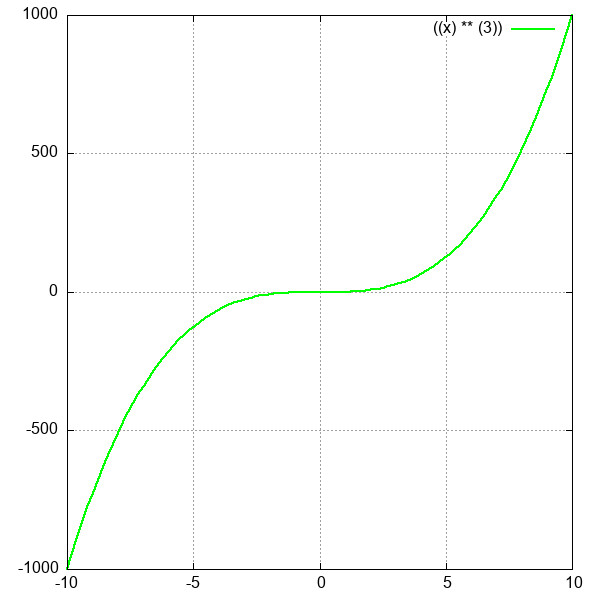
\includegraphics{GraphicDumps/plot.jpg}\newpage \textbf{\LARGE Глава II. Визуальный анализ функции}

Очевидно, что

\begin{center}
$y = $$x^{3}$

\end{center}
\newpage \textbf{\LAGRE Глава III. Дифференцирование}

Паршивая функция всё доказательство портит

\begin{center}
 ($x)'
  = 1$\end{center}
[Данные удалены]

\begin{center}
 ($3)'
  = 0$\end{center}
Господи, да для кого я вообще стараюсь

\begin{center}
 ($x^{3})'
  = (x^{3} \cdot ((\frac{3}{x} \cdot 1) + (0 \cdot log(x))))$\end{center}
\newpage \textbf{\LARGE Глава IV.Упрощение выражения}

Спешка нужна только в армии и при ловле блох. Но не как уж ни при вычислении производной

\begin{center}
$(\frac{3}{x} \cdot 1) = \frac{3}{x}$\end{center}
Segmentation fault (core dumped)

\begin{center}
$(0 \cdot log(x)) = 0$\end{center}
Если вы не понимаете этот переход, то я вам сочувствую

\begin{center}
$(\frac{3}{x} + 0) = \frac{3}{x}$\end{center}
\newpage \textbf{\LARGE Глава V. Полученая производная}

$y = $$x^{3}$

$y' = $$(x^{3} \cdot \frac{3}{x})$

\includegraphics{GraphicDumps/plot_1.jpg}
\end{document}